% --------------------------------------------------------------
% 改進後的 LaTeX 報告模板
% --------------------------------------------------------------
\documentclass[12pt]{article}

\usepackage[margin=1in]{geometry}
\usepackage{amsmath, amssymb, amsthm}
\usepackage{graphicx}
\usepackage{subcaption} % 用於多張圖片對齊
\usepackage{booktabs}   % 用於表格格式化
\usepackage[colorlinks = true, urlcolor = blue, linkcolor = black, citecolor = black]{hyperref}
\usepackage[backend=biber,style=ieee]{biblatex} % 文獻引用
\usepackage{bbding} 
\usepackage[width=.8\textwidth]{caption} % Make table caption width the same w/ table
\usepackage{xeCJK}
    \setCJKmainfont[AutoFakeBold=3]{AR PL UKai TW}
    \XeTeXlinebreaklocale "zh"             
    \XeTeXlinebreakskip = 0pt plus 1pt
\usepackage{titlesec}
\usepackage{listings}
\usepackage{xcolor}

% Define colors for syntax highlighting
\definecolor{codegreen}{rgb}{0,0.6,0}     % 註解 (綠色)
\definecolor{codegray}{rgb}{0.5,0.5,0.5}  % 行號 (灰色)
\definecolor{codepurple}{rgb}{0.58,0,0.82} % 字串 (紫色)
\definecolor{backcolour}{rgb}{0.95,0.95,0.92} % 背景色
\definecolor{keywordblue}{rgb}{0,0,1}     % 關鍵字 (藍色)
\definecolor{classred}{rgb}{0.8,0,0}      % 類別 (紅色)

% Configure listings style
\lstdefinestyle{mystyle}{
    backgroundcolor=\color{backcolour},   
    commentstyle=\color{codegreen},        % 註解顏色
    keywordstyle=\color{keywordblue},      % 關鍵字 (如 def, class)
    numberstyle=\tiny\color{codegray},     % 行號顏色
    stringstyle=\color{codepurple},        % 字串顏色
    basicstyle=\ttfamily\footnotesize,     % 字體設定
    breakatwhitespace=false,         
    breaklines=true,                       
    captionpos=t,                         
    keepspaces=true,                       
    numbers=left,                          
    numbersep=5pt,                         
    showspaces=false,                      
    showstringspaces=false,                
    showtabs=false,                        
    tabsize=4,                             
    frame=single,                          % 單線框
    morekeywords={self},                    % 強調 Python 的 self
    emph={class}, emphstyle=\color{classred} % 讓 class 變紅色
}

% Set default style
\lstset{style=mystyle}

% 文獻引用檔案
\addbibresource{references.bib}

\begin{document}


\title{AI-Capstone: Project1 Report}
\author{111550093 朱驛庭}
\maketitle


\section{Introduction}
In this project, our objective is to classify images of clothing items into predefined categories using various machine learning techniques. The task involves implementing and comparing the performance of three different models: ResNet, a deep learning-based approach; K-means, an unsupervised learning method; and SVM, a traditional supervised learning algorithm. The goal is to evaluate the effectiveness of these models in accurately classifying clothing items based on their visual characteristics.

\section{Dataset}  
The dataset used in this project comprises clothing item images collected from Google Search and Unsplash. It is shared with a classmate (student ID: 111550160). The dataset can be accessed through the \href{https://github.com/ChuEating1005/AI-Capstone/tree/main/Project1/images}{link (click)}.

    \subsection{Source}
    To assess the generalization capabilities of different models, the dataset includes images with varying levels of similarity within each category. For example, some images feature models wearing clothing items, while others showcase only clothing. The dataset comprises ten clothing categories: T-shirt, bag, dress, glasses, hat, hoodie, jacket, pants, shoes, and socks, with 50 images per category, totaling 500 images.
    
    \subsection{Train-test Split}
    The dataset is divided into training and testing sets, with 80\% of the data used for training and 20\% for testing. This split ensures that the models are trained on a substantial amount of data while retaining a separate set for evaluating their performance.

    \subsection{Preprocessing}
    I organized the images into separate folders based on their respective categories, naming each folder after the corresponding clothing type. Additionally, all images were converted to JPG format and sequentially renamed from 1 to 50.
    
\section{Methods}  
    \subsection{Supervised Method1: Support Vector Machine}  
    Support Vector Machine (SVM) is a supervised learning algorithm designed to find the optimal hyperplane that best separates data into different classes while maximizing the margin between them. The margin is defined as the distance between the hyperplane and the closest data points, known as \textbf{support vectors}. A larger margin generally leads to better generalization and robustness against overfitting. The illustration is show in Fig.~\ref{fig:svm}. The SVM classifier seeks to minimize the following objective function:  
    \begin{equation*}
        \min_{w, b} \frac{1}{2} \|w\|^2 \quad \text{s.t. } y_i (w^T x_i + b) \geq 1, \forall i
    \end{equation*}  
    where \( w \) represents the weight vector, \( b \) is the bias term, \( x_i \) denotes the input feature vector, and \( y_i \) is the corresponding class label (\(+1\) or \(-1\)).
    
    \begin{figure}[h]
        \centering
        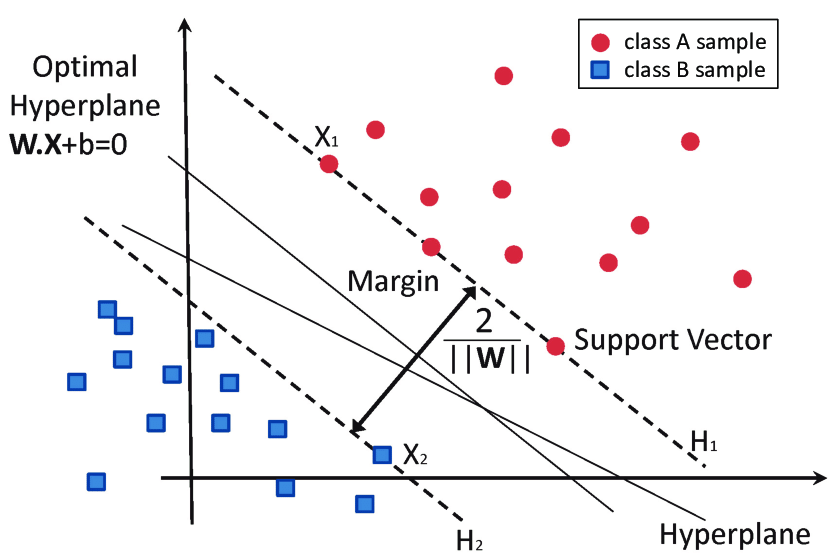
\includegraphics[width=0.6\textwidth]{svm.png}
        \caption{SVM Illustration \cite{svm_medium}.} 
        \label{fig:svm}
    \end{figure}
    
        \subsubsection{Hinge Loss and Soft Margin SVM}  
        To handle cases where data points may not be perfectly separable, SVM introduces \textbf{soft margin classification}, allowing for certain misclassifications by incorporating \textbf{slack variables} \( \xi_i \). This is achieved by optimizing the \textbf{hinge loss function}, which penalizes misclassified points:  
        \begin{equation*}
            \min_{w, b, \xi} \frac{1}{2} \|w\|^2 + C \sum_{i=1}^{n} \xi_i
        \end{equation*}  
        subject to:  
        \begin{equation*}
            y_i (w^T x_i + b) \geq 1 - \xi_i, \quad \xi_i \geq 0, \forall i
        \end{equation*}  
        where \( C \) is a regularization parameter that balances the trade-off between maximizing the margin and minimizing classification errors.
    
        \subsubsection{Kernel Trick for Non-Linearly Separable Data}
        When the data is not linearly separable in the original feature space, SVM leverages the \textbf{kernel trick} to project the data into a higher-dimensional space where it becomes linearly separable. The kernel function replaces the direct computation of dot products, effectively mapping data into a transformed feature space:  
        \begin{equation*}
            K(x_i, x_j) = \phi(x_i)^T \phi(x_j)
        \end{equation*}  
        where \( \phi(x) \) is a mapping function that transforms the input space into a higher-dimensional feature space.
    
        \subsection{Supervised Method2: ResNet18}  
        ResNet18 is a deep convolutional neural network (CNN) that belongs to the ResNet (Residual Network) family, introduced by He et al. in 2015. It is designed to address the vanishing gradient problem in deep networks by incorporating residual connections, allowing for deeper architectures while maintaining efficient training. ResNet18 consists of 18 layers, including convolutional, batch normalization, ReLU activation, and fully connected layers.
    
           \subsubsection{Architecture and Modification}  
            ResNet18 follows a hierarchical structure with an initial convolutional layer, followed by 8 residual blocks grouped into 4 stages, and ending with a global average pooling and a fully connected layer. The modified version in this project replaces the original 1000-class output layer with a fully connected layer of size 10, corresponding to our clothing categories. The softmax activation is removed to output raw logits, which are processed by a cross-entropy loss function. The modified final layer is defined as:
            \begin{equation*}
                \text{FC Layer: } y = Wx + b, \quad W \in \mathbb{R}^{10 \times 512}, \quad b \in \mathbb{R}^{10}
            \end{equation*}
            The overall structure of ResNet18 is illustrated in Fig.~\ref{fig:resnet18}.
            \begin{figure}[h]
                \centering
                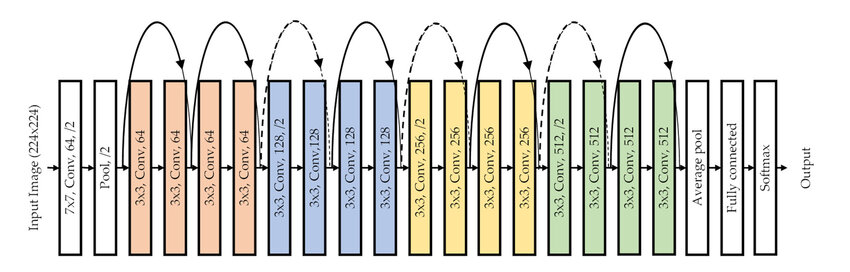
\includegraphics[width=0.8\textwidth]{resnet18_structure.png}
                \caption{Structure of the ResNet18 Model \cite{resnet18_figure}.} 
                \label{fig:resnet18}
            \end{figure}
    
            \subsubsection{Loss Function}  
            The model is trained using the \textbf{cross-entropy loss function}, defined as:
            \begin{equation*}
                L_{\text{CE}} = - \sum_{i=1}^{N} \left[ y_i \log p_i + (1 - y_i) \log (1 - p_i) \right]
            \end{equation*}
            where \( y_i \) is the true class label, \( p_i \) is the predicted probability, and \( N \) is the total number of samples.    
    
    \subsection{K-Means Clustering}  
    K-Means is a widely used unsupervised learning algorithm for clustering, aiming to partition a dataset into \( K \) clusters based on feature similarity. It operates iteratively to minimize intra-cluster variance, ensuring that data points within a cluster are as close as possible to the cluster centroid. The objective function, known as the \textbf{within-cluster sum of squares (WCSS)}, is given by:  
    \begin{equation*}
    \sum_{j=1}^{K} \sum_{i \in C_j} \| x_i - c_j \|^2
    \end{equation*}  
    where \( C_j \) represents the set of data points assigned to cluster \( j \), and \( c_j \) is the centroid of that cluster.

\section{Implementation Details}
    \subsection{Evaluation Metrics}
        \subsubsection{Supervised Methods}
        For the supervised methods, namely ResNet and SVM, I employ several evaluation metrics to assess the performance of the models:
        
        \begin{itemize}
            \item \textbf{Confusion Matrix}: A confusion matrix is used to visualize the classification model's performance by organizing predictions into four categories:
            \[
            \begin{bmatrix}
            TP & FP \\
            FN & TN
            \end{bmatrix}
            \]
            where:
            \begin{itemize}
                \item \textbf{True Positives (TP)}: Correctly predicted positive instances.
                \item \textbf{False Positives (FP)}: Incorrectly predicted positive instances.
                \item \textbf{False Negatives (FN)}: Incorrectly predicted negative instances.
                \item \textbf{True Negatives (TN)}: Correctly predicted negative instances.
            \end{itemize}

            \item \textbf{Accuracy}: This metric measures the proportion of correctly classified instances over the total number of instances, providing a general sense of model performance. It is defined as:
            \begin{equation*}
                \text{Accuracy} = \frac{TP + TN}{TP + TN + FP + FN}
            \end{equation*}
    
            \item \textbf{Precision}: Precision measures the proportion of correctly predicted positive instances among all instances classified as positive. It is given by:
            \begin{equation*}
                \text{Precision} = \frac{TP}{TP + FP}
            \end{equation*}
        
            \item \textbf{Recall (Sensitivity)}: Recall measures the model's ability to correctly identify all actual positive instances. It is calculated as:
            \begin{equation*}
                \text{Recall} = \frac{TP}{TP + FN}
            \end{equation*}
            
            \item \textbf{F1-Score}: The F1-score is the harmonic mean of precision and recall, balancing the trade-off between them. It is defined as:
            \begin{equation*}
                \text{F1-Score} = \frac{2 \times \text{Precision} \times \text{Recall}}{\text{Precision} + \text{Recall}}
            \end{equation*}
        \end{itemize}
        These metrics are computed using the \texttt{classification\_report} function from scikit-learn, providing a comprehensive overview of the model’s performance across different classes.
        
    
        \subsubsection{Unsupervised Method}
        For the unsupervised method, K-means, I use different metrics to evaluate clustering performance:
        \begin{itemize}
            \item \textbf{Silhouette Score}: This metric measures how similar an object is to its own cluster compared to other clusters. It ranges from -1 to 1, where a higher score indicates better-defined clusters.
            \item \textbf{Adjusted Rand Index (ARI)}: ARI measures the similarity between the clustering results and the true labels, adjusted for chance. It ranges from -1 to 1, with 1 indicating perfect agreement.
            \item \textbf{Calinski-Harabasz Score}: This metric evaluates the ratio of between-cluster dispersion to within-cluster dispersion. A higher score indicates well-separated and compact clusters.
            \item \textbf{Davies-Bouldin Score}: This metric assesses the average similarity between each cluster and its most similar cluster. A lower score indicates better clustering quality, as it suggests that clusters are well-separated.
        \end{itemize}
    
    \subsection{Hyperparameters}
    \begin{itemize}
        \item \textbf{ResNet}: The ResNet model's hyperparameters are carefully chosen to ensure effective training and convergence. The learning rate is initialized at 0.001, and a \texttt{StepLR} scheduler is used to dynamically adjust the learning rate during training. This scheduler reduces the learning rate by a factor of 0.1 every 10 epochs, helping the model converge more smoothly. The random seed is set to 40 to ensure reproducibility of results. The model is initialized with weights pre-trained on the ImageNet dataset, which provides a strong starting point for feature extraction. The batch size is set to 32, and the model is trained for 20 epochs, balancing computational efficiency with model performance.
    
        \item \textbf{SVM}: For the SVM model, I perform a grid search over a range of hyperparameters, including the regularization parameter \( C \), kernel type (e.g., \texttt{rbf}, \texttt{poly}), and kernel-specific parameters like gamma and degree. This search is conducted using \texttt{GridSearchCV} from scikit-learn, which performs cross-validation to find the optimal hyperparameter combination.
    
        \item \textbf{K-means}: The primary hyperparameter for K-means is the number of clusters \( K \). I experiment with different values of \( K \) and use the ARI score to select the optimal number of clusters. Additionally, I use UMAP for dimensionality reduction before clustering, which involves tuning the number of components and the minimum distance between points.
    \end{itemize}

\section{Experiments}
    \subsection{Data Augmentation}
    Data augmentation is a technique commonly used in machine learning to artificially expand the training dataset by applying transformations to the input images. The key idea is that by introducing non-identical inputs to the model in each epoch, data augmentation helps prevent overfitting and improves the generalization ability of the model. This is particularly beneficial for deep learning models, which tend to overfit when trained on small datasets. The comparison is shown below:
    \begin{table}[h]
        \centering
        \renewcommand{\arraystretch}{1.2}
        \begin{tabular}{cc|c c c c}
            \toprule
            Methods & Aug. & Accuracy(\%) & Precision(\%) & Recall(\%) & F1-score(\%) \\
            \midrule
            SVM & \XSolidBrush  & \textbf{73.74} & \textbf{76.30} & \textbf{73.80} & \textbf{73.80} \\
            SVM & \Checkmark & 69.70 & 70.70 & 69.70 & 69.30 \\
            \midrule
            ResNet18 & \XSolidBrush & 86.87 & 89.60 & 86.80 & 86.80 \\
            ResNet18 & \Checkmark & \textbf{91.92} & \textbf{92.50} & \textbf{91.80} & \textbf{91.70} \\
            \bottomrule
        \end{tabular}
        \caption{Performance comparison of the effect of data augmentation on the two supervised methods.}
        \label{tab:data_aug_results}
    \end{table}
    \begin{figure}[h]
        \centering
        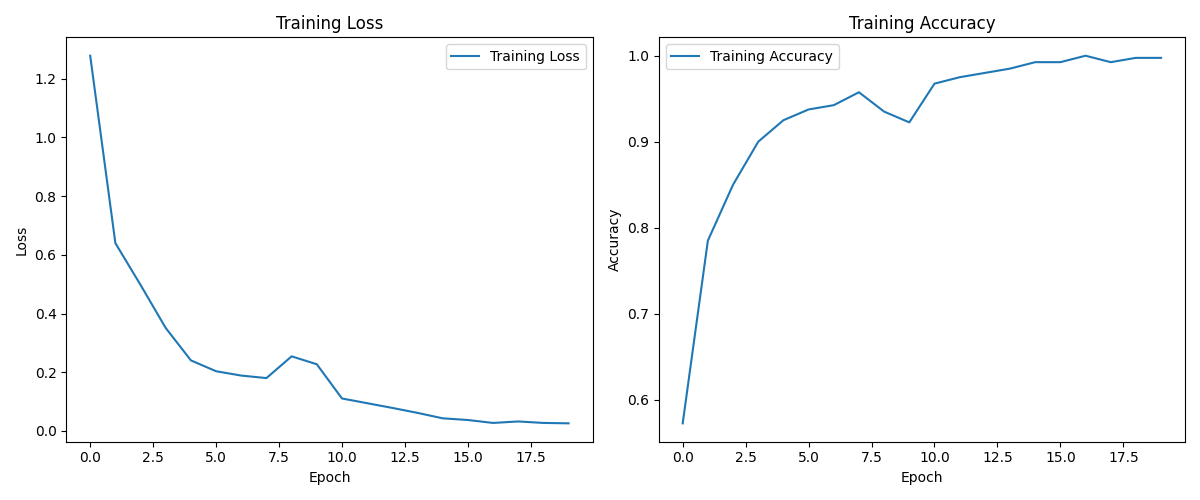
\includegraphics[width=0.8\textwidth]{figure/resnet_aug_training_history.png}
        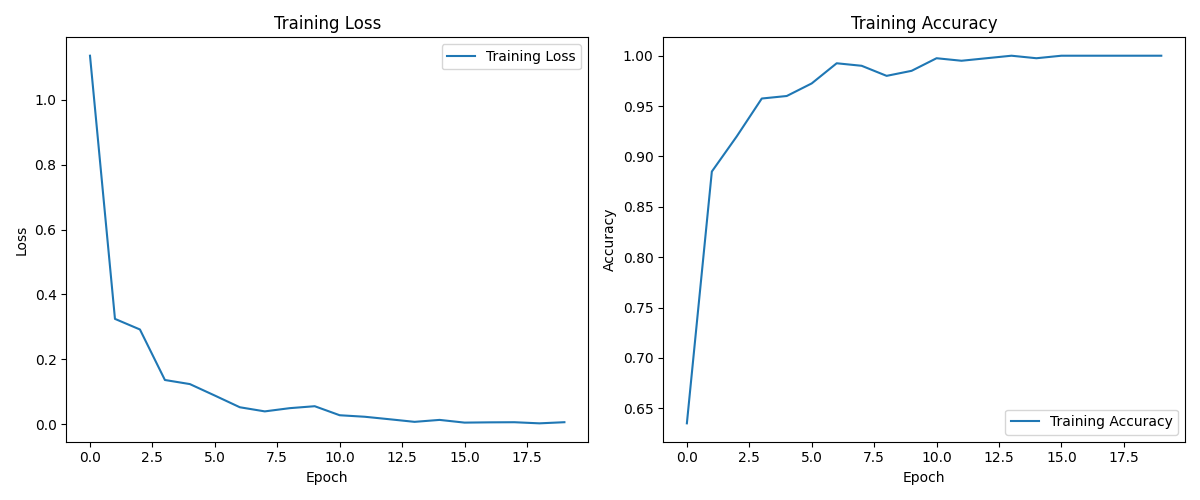
\includegraphics[width=0.8\textwidth]{figure/resnet_ori_training_history.png}
        \caption{Training history of ResNet18 with and without data augmentation. The top row represents training with data augmentation, while the bottom row represents training without it.} 
        \label{fig:training_history_resnet}
    \end{figure}\\
    From the results presented in Table~\ref{tab:data_aug_results}, it is evident that data augmentation enhances the performance of ResNet18. This improvement suggests that ResNet18 benefits from the increased diversity introduced by augmentation, allowing it to generalize better to unseen data. However, the same approach does not yield positive results for SVM, as it is not a deep learning-based method. Instead of improving performance, the additional variations introduced by data augmentation negatively impact SVM, likely due to its reliance on handcrafted features rather than learned representations.\\[5pt]
    Furthermore, as shown in Figure~\ref{fig:training_history_resnet}, data augmentation slows down the training process compared to the original setup. The model takes longer to converge since it needs to learn from a more diverse set of augmented samples. In typical cases, data augmentation may require additional training epochs to reach the same level of training loss as a model trained without augmentation.

    \subsection{t-SNE Visualization on ResNet18}
    t-SNE (t-distributed stochastic neighbor embedding) is a dimensionality reduction technique commonly used for visualization. By mapping high-dimensional data into a lower-dimensional space, t-SNE helps reveal underlying patterns and relationships within the data. In Figure~\ref{fig:tsne_resnet}, we observe that as the data progresses through each layer of ResNet, the separation between different classes becomes more distinct. Notably, in the fully connected layer, the \textit{hoodie}, \textit{jacket}, and \textit{t-shirt} classes are positioned relatively close to one another. This alignment is reasonable, as these three types of clothing share similar visual characteristics in the real world.
    \begin{figure}[h]
        \centering
        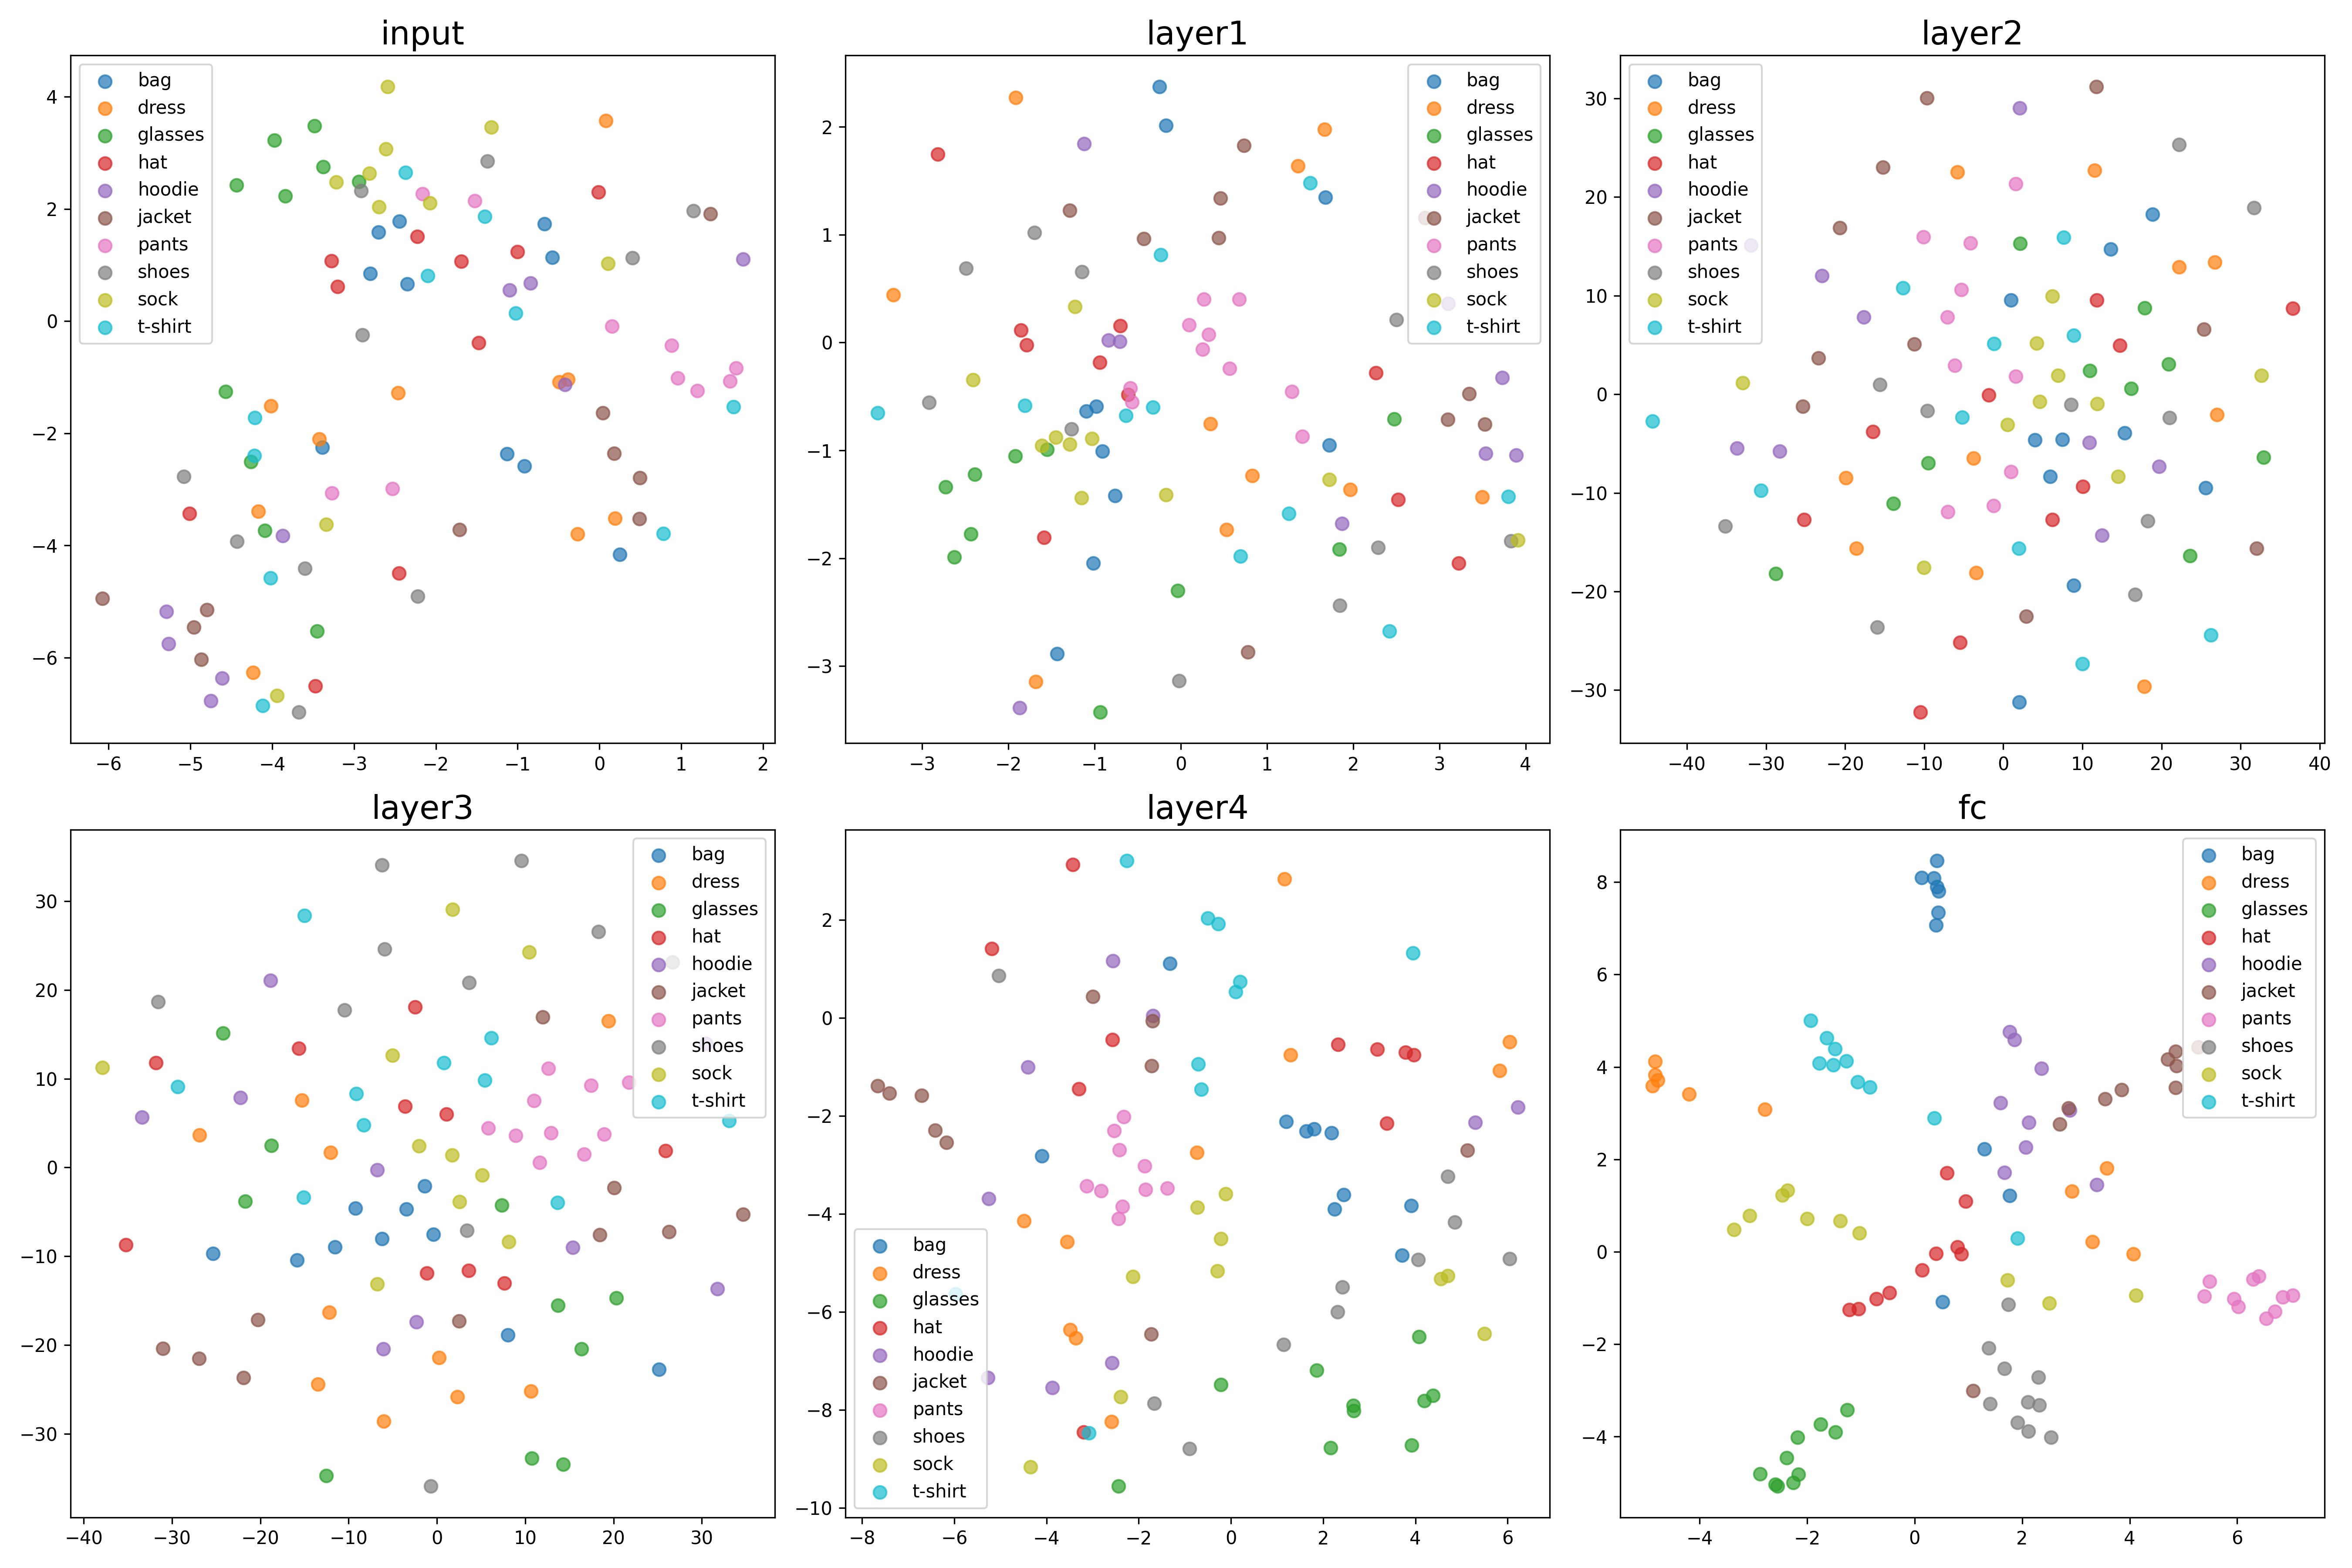
\includegraphics[width=0.8\textwidth]{figure/resnet_tsne_comparison.png}
        \caption{t-SNE visualization of different layers on ResNet18.} 
        \label{fig:tsne_resnet}
    \end{figure}

    \subsection{Multi-criteria Cluster Validation of K-means}
    Based on the result shown on Figure.~\ref{fig:kmeans_metrics}. The analysis of K-means clustering metrics suggests that K=5 or K=6 provides the best balance across multiple validation metrics. The \textbf{Silhouette Score} and \textbf{Calinski-Harabasz Score} indicate that K=5 achieves strong separation, while K=6 has the highest \textbf{Adjusted Rand Index (ARI)}, suggesting better alignment with true labels. The \textbf{Davies-Bouldin Score} further supports K=5 or K=6 as optimal choices. At K=6, some clusters achieve high purity, such as bags (77.78\%) and glasses (40.74\%), while upper-body garments (t-shirts, jackets, and hoodies) tend to mix. The results indicate that while K-means effectively groups certain categories, visual similarities between some clothing items limit perfect separation. For general clothing classification, K=5 or K=6 is recommended, while K=2 or K=3 may suffice for broader category distinctions.
    \begin{figure}[h]
        \centering
        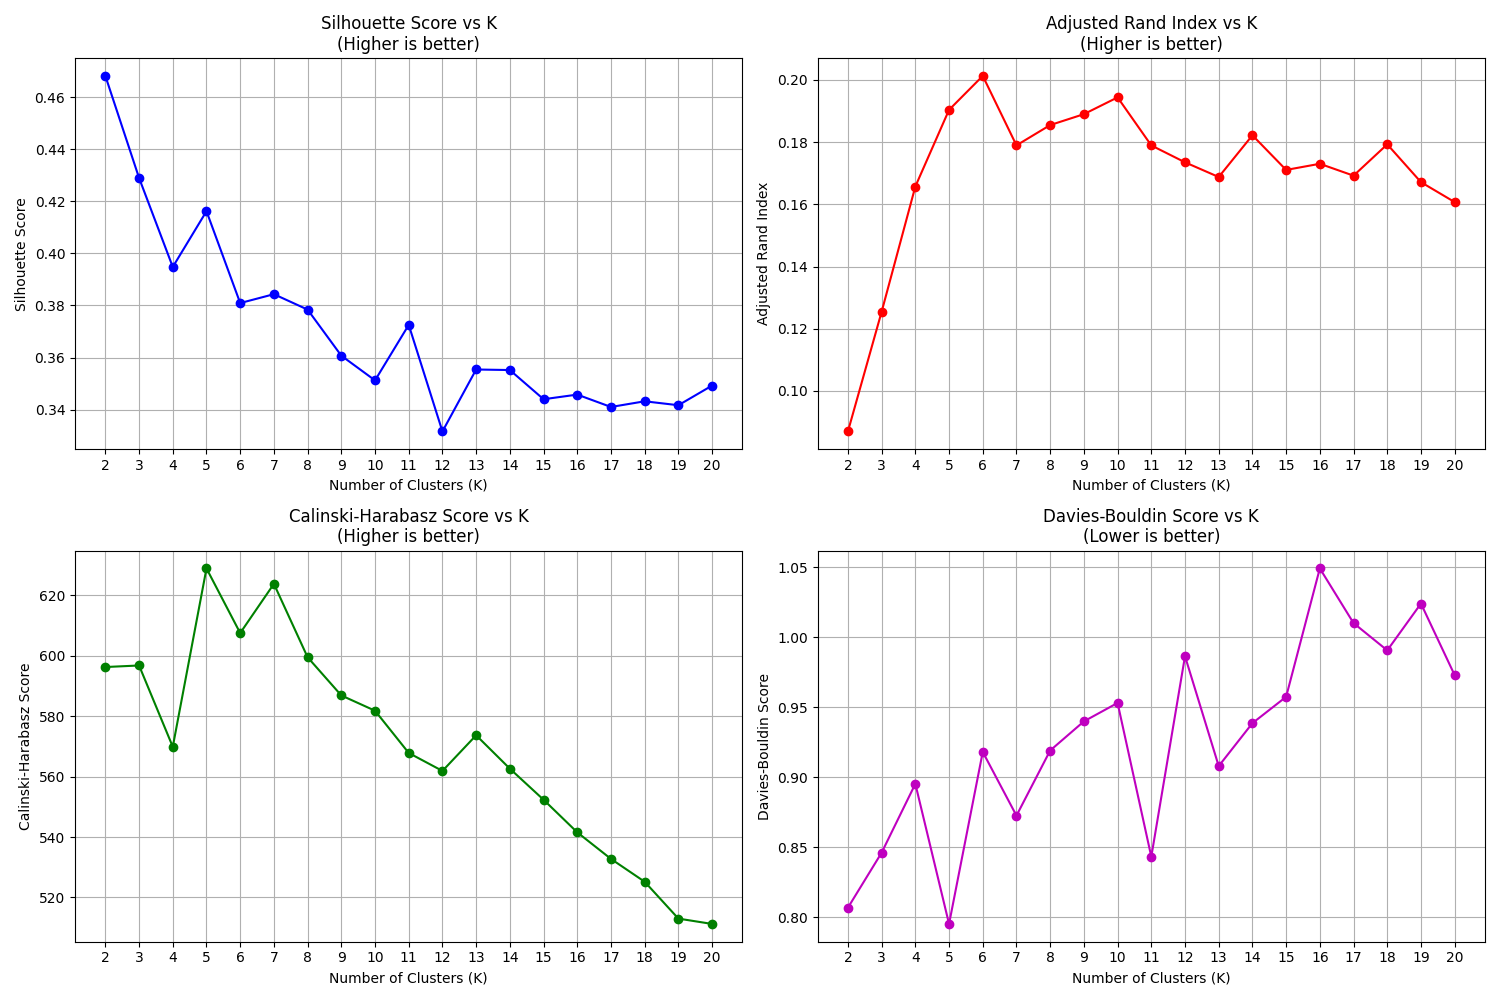
\includegraphics[width=0.8\textwidth]{figure/kmeans_metrics_comparison.png}
        \caption{K-means clustering evaluation metrics for different numbers of clusters (K).} 
        \label{fig:kmeans_metrics}
    \end{figure}
    
\section{Discussion}
    \subsection{Performance Comparison and Analysis}
    In this project, I have implemented and evaluated three different machine learning approaches for clothing image classification: ResNet18, SVM, and K-means. The experiments yielded several interesting observations:
    
    \begin{itemize}
        \item \textbf{ResNet18} demonstrated superior performance with a test accuracy of 91.92\% when using data augmentation, outperforming the other methods. This result aligns with expectations, as deep learning methods typically excel at image classification tasks due to their ability to learn hierarchical representations directly from raw pixel data.
        
        \item \textbf{SVM} achieved a respectable accuracy of 73.74\% without data augmentation. Interestingly, data augmentation decreased its performance, contradicting the common assumption that augmentation universally improves classification results. This suggests that traditional machine learning algorithms like SVM may struggle with the increased variance introduced by augmentation when using handcrafted features.
        
        \item \textbf{K-means}, as an unsupervised approach, showed limitations in perfectly separating the clothing categories, achieving a maximum ARI of 0.20 at K=6. This was expected, as unsupervised methods lack the guidance of class labels during training. However, the clustering revealed meaningful patterns, particularly in separating accessories from clothing items.
    \end{itemize}
    
    \subsection{Factors Affecting Performance}
    Several factors influenced the performance of the different models:
    
    \begin{itemize}
        \item \textbf{Feature Representation}: ResNet18's superior performance can be attributed to its ability to learn complex, hierarchical features directly from raw images. In contrast, SVM relied on manually engineered features, which, while effective, may not capture all the nuances present in the data.
        
        \item \textbf{Dataset Characteristics}: The dataset's inherent challenges, such as varying backgrounds, lighting conditions, and item orientations, affected all models. Items with distinctive shapes (like bags) were generally easier to classify or cluster correctly compared to items with similar appearances (like t-shirts, hoodies, and jackets).
        
        \item \textbf{Visual Similarity}: The t-SNE visualization and K-means clustering results both revealed that visually similar categories (such as hoodie, jacket, and t-shirt) tend to overlap in the feature space. This suggests that even with sophisticated feature extraction, some ambiguity between similar clothing categories is inevitable.
        
        \item \textbf{Dimensionality Reduction}: For K-means, the UMAP dimensionality reduction played a crucial role in clustering performance. The optimal number of dimensions balanced between preserving data structure and reducing noise.
    \end{itemize}
    
    \subsection{Lessons Learned}
    Overall, this project demonstrates the complementary nature of different machine learning approaches for image classification tasks. Each method offers unique insights and advantages, with deep learning-based approaches like ResNet18 providing state-of-the-art performance, traditional methods like SVM offering interpretability and computational efficiency, and unsupervised methods like K-means revealing natural data patterns without requiring labeled data.

\printbibliography % 輸出文獻

\newpage

\appendix
\titleformat{\section}{\Large\bfseries}{Appendix}{0.5em}{} 

\section{}
Github link: \href{https://github.com/ChuEating1005/AI-Capstone/tree/main/Project1}{https://github.com/ChuEating1005/AI-Capstone/tree/main/Project1}
\lstinputlisting[language=Python, caption={prepare\_dataset.py}]{code/prepare_dataset.py}
\lstinputlisting[language=Python, caption={dataset.py}]{code/dataset.py}
\lstinputlisting[language=Python, caption={main.py}]{code/main.py}
\lstinputlisting[language=Python, caption={models/ResNet.py}]{code/ResNet.py}
\lstinputlisting[language=Python, caption={models/SVM.py}]{code/SVM.py}
\lstinputlisting[language=Python, caption={models/K\_means.py}]{code/K_means.py}

\end{document}